\chapter{Evaluation}
\section{Planning for future work}
By the time of submission of this report, there are still several primary components that require completion. 
The machine Learning model requires proper optimisation and actual field tests to identify primary weaknesses and computational losses. 
There is a high possibility of studying CUDA programming to increase the efficiency of overall detection and playthrough performance.
The Raspberry Pi communication still requires integration with actual tank control. Also, it will be part of another research to investigate the possibility of using their own R-Pi 360 camera or NFC communication module.
Nevertheless, the problem with detection was already resolved gracefully using advanced techniques, maybe some of those problems will be overcome as well using parallel computing, CUDA usage and some creative thinking.
\subsection{Research Problems}
This research aimed to introduce an unusual way of approaching Augmented reality, defined in a simple tank commander simulation game in a closed arena scale. The main difficulty is the scope of limitations and unknown expectations due to equipment possibilities. Despite the difficulty of reconstructing a real environment in virtual, such computer graphics require a much more powerful computational system. 
Besides, the game experience itself is slower with possessed equipment, so some implementations may postpone themselves for later. \\
\newpage
\begin{landscape}
\section{Timeline for completion}	
\textbf{Probably add two of them}
	Figure~\ref{fig:chart} below represents the Final version of tasks and the percentage of completion.
    It defines requirements established by the Work Integrated Learning (WIL) department, progress reports and assessments, project time-frames and supervisor expectations.
    There should be no more changes to the provided chart any further.
	\begin{figure}[H]
		\centering
		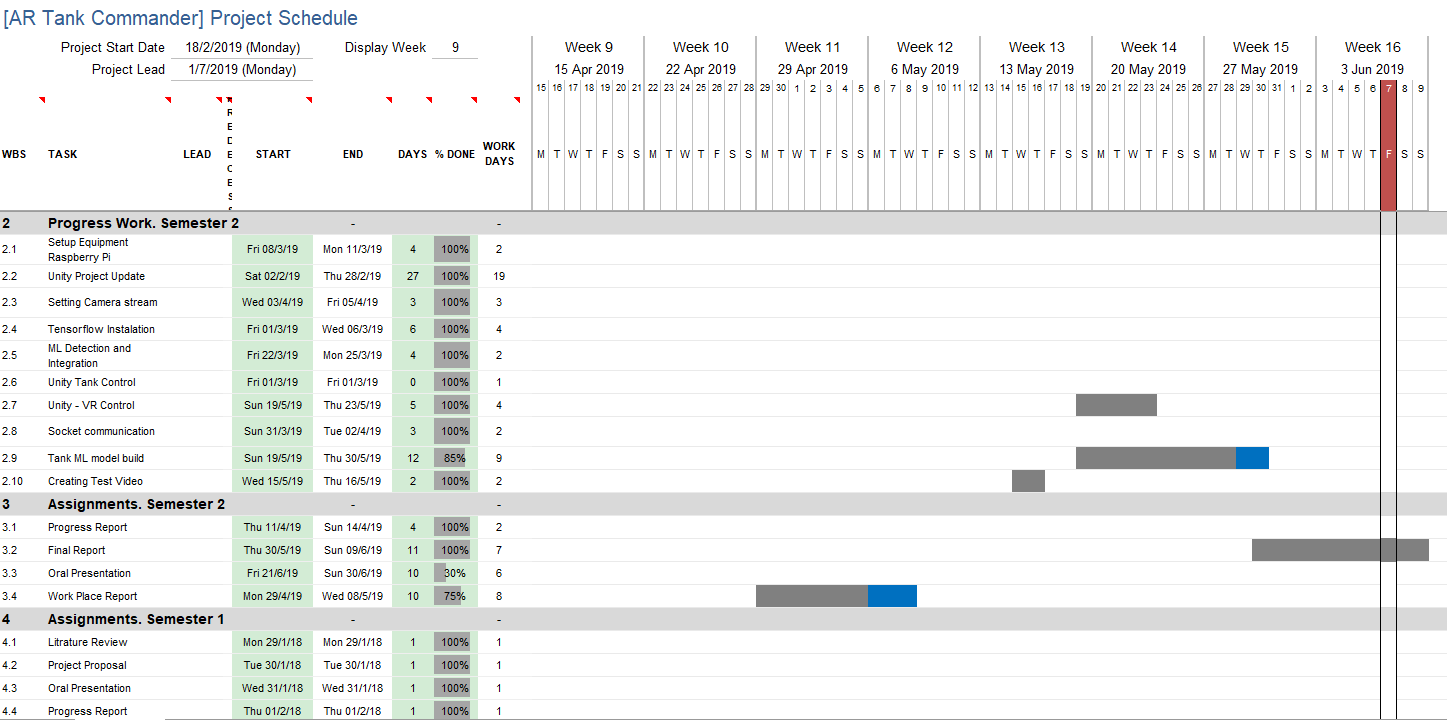
\includegraphics[width=0.8\linewidth]{evaluation/charts/chart3.PNG}
		\caption{Final Project Schedule}
		\label{fig:chart}
	\end{figure}		
\end{landscape}